%%%%%%%%%%%%%%%%%%%%%%%%%%%%%%%%%%%%%%%%%%%%%%%%%
%%%%%  make IFJtalk13.pdf
%%%%%%%%%%%%%%%%%%%%%%%%%%%%%%%%%%%%%%%%%%%%%%%%%
\documentclass{beamer}
%\documentclass[handout]{beamer}


\mode<presentation>
{
  \usetheme{Warsaw}
 %\usetheme{Hannover}
  \setbeamercovered{transparent}
}

\usepackage[english]{babel}
\usepackage{xcolor}
\usepackage[latin1]{inputenc}

\usepackage{times}
\usepackage[T1]{fontenc}
\usepackage{listings}
%------------------------------------------------------
\usepackage{amsbsy}
\usepackage{amsmath,amssymb,bbm}
\usepackage{euscript}
\usepackage{fancybox}


%%%%%%%%%%%%%%%%%%%%%%%%%%%%%%%%%%%%%%%%%%%%%%%%%%%%%%%%%%%%%%%
%%% Macros 
\newcommand{\Pcal}{{\cal P}}
\newcommand{\Kcal}{{\cal K}}
\newcommand{\Dcal}{{\cal D}}
%
\newcommand{\Peu}{\EuScript{P}}
\newcommand{\Keu}{\EuScript{K}}
\newcommand{\Deu}{\EuScript{D}}
\newcommand{\Reu}{\EuScript{R}}
\newcommand{\Feu}{\EuScript{F}}
%
\newcommand{\Pmf}{\mathfrak{P}}
\newcommand{\Dmf}{\mathfrak{D}}
%
\newcommand{\Pbbm}{\mathbbm{P}}
\newcommand{\Rbbm}{\mathbbm{R}}
\newcommand{\Zbbm}{\mathbbm{Z}}
\newcommand{\Bbbm}{\mathbbm{B}}
\newcommand{\Pop}{\overleftarrow{\Pbbm}}
\newcommand{\Zop}{\overleftarrow{\Zbbm}}
\newcommand{\Bop}{\overleftarrow{\Bbbm}}
\newcommand{\Rop}{\overleftarrow{\Rbbm}}
%
\newcommand{\Tbf}{\mathbf{T}}
\newcommand{\Pbf}{\mathbf{P}}
\newcommand{\Dbf}{\mathbf{D}}
\newcommand{\Phibf}{\mathbf{\Phi}}
%
\newcommand{\udl}{\underline}
\newcommand{\from}{\leftarrow}
\newcommand{\bu}{\bullet}
\newcommand{\veps}{\varepsilon}
\newcommand{\Dyfs}{D_{_{\rm YFS}}}
\newcommand{\tH}{{\hat{t}}}
\newcommand{\tB}{{\bar{t}}}
\newcommand{\tBl}{{\bar{t}_\lambda}}
% boldfaces and vectors
\newcommand{\ba}{{\bf{a}}}
\newcommand{\bk}{{\bf{k}}}
\newcommand{\vkap}{{\vec{\kappa}}}
\newcommand{\vrk}{{\varkappa}}
\newcommand{\alfb}{{\bar{\alpha}}}
\newcommand{\betb}{{\bar{\beta}}}


\newcommand{\cbl}{\color{blue}}
\newcommand{\crd}{\color{red}}
\newcommand{\cmg}{\color{magenta}}
\newcommand{\cgr}{\color{green}}
\newcommand{\cwh}{\color{white}}
\newcommand{\yel}{\color{yellow}}
\newcommand{\blk}{\color{black}}
\newcommand{\cya}{\color{cyan}}

\newcommand{\ns}{\normalsize}

%%%%%%%%%%%%%%%%%%%%%%%%%%%%%%%%%%%%%%%%%%%%%%%%%%%%%%%%%%%%%%%%%%%%%%%%
%%%%%%%%%%%%%%%%%%%%%%%%%%%%%%%%%%%%%%%%%%%%%%%%%%%%%%%%%%%%%%%%%%%%%%%%
%%%%%%%%%%%%%%%%%%%%%%%%%%%%%%%%%%%%%%%%%%%%%%%%%%%%%%%%%%%%%%%%%%%%%%%%
%%%%%%%%%%%%%%%%%%%%%%%%%%%%%%%%%%%%%%%%%%%%%%%%%%%%%%%%%%%%%%%%%%%%%%%%
\title[Monte Carlo Methods] % (optional)
{ {\bf KKMC -- Status and Outlook}
} % (optional)


\author[S.~Jadach] % (optional, use only with lots of authors)
{\Large\bf S.~JADACH 
   \\
   \normalsize in collaboration with B.F.L. Ward and Z. W\c{a}s}


\institute[Universities of Somewhere and Elsewhere] % (optional)
{ {\large\crd IFJ-PAN, Krak\'ow, Poland}\\
  {~~~}\\
  {\footnotesize
  Partly supported by Polish Government grant\\
  {\em Narodowe Centrum Nauki} DEC-2011/03/B/ST2/02632
}}

\date[Short Occasion] % (optional)
{\small Workshop on 
   tau lepton decays: hadronic currents from data of  Belle and BaBar 
   and new physics signatures at LHC\\
   Krakow,
   September 15-20th, 2013
\vskip 4mm
 \footnotesize
  More material on
  http://jadach.web.cern.ch/
}

\subject{Talks}
% only for the PDF information catalog.

\pgfdeclareimage[height=0.5cm]{university-logo}{ifj}
\logo{\pgfuseimage{university-logo}}


\begin{document}

\begin{frame}
  \titlepage
\end{frame}
%----------------------------------------------------------------------
%----------------------------------------------------------------------
%----------------------------------------------------------------------


%----------------------------------------------------------------------
\begin{frame}[fragile]
\frametitle{\bf What is KKMC?}
{\large
KKMC is the MC event generator for the process:\\
~~~~~~~~~~~~~~\fbox{\cbl $e^-e^+ \to f\bar{f}+ n\gamma$}\\
{\cbl $f=\mu,\tau,\nu,u,d,s,c,b$,~~~~ $n=0,1,2...\infty$.}
}\\
Interfaced with TAUOLA+PHOTOS\\
and with electroweak library DIZET.\\

Published version \fbox{\cmg 4.13} (to be cited):
\begin{itemize}
\item
Comput.Phys.Commun. 130(2000) 360, hep-ph/9912214,\\
F77 code description and user guide (manual).
\item
Phys. Rev. D63 (2001) 113009, hep-ph/0006359\\
physics content, CEEX exponentiation of QED corrs.\\
\end{itemize}
"Workhorse" in data analysis of all four LEP collaborations.\\
~~~\\
\footnotesize
(Replacement of earlier MC's KORALZ and KORALB.)\\
(Not aplicable for  $e^-e^+ \to e^-e^+$)

\end{frame}
%----------------------------------------------------------------------

%----------------------------------------------------------------------
\begin{frame}[fragile]
\frametitle{\bf More KKMC versions available since 2000}
\framesubtitle{http://jadach.web.cern.ch/jadach/KKindex.html}
\small
\begin{itemize}
\item
Production Version \fbox{\cmg 4.16}, Oct. 2001,  
(KKMC-v.4.16d-export.tar.gz).
Improved $\nu\bar{\nu}$ matrix elm.\\
RRes module for $\gamma^* \to narrow~resonances$ at LEP.
\item
Developement Version \fbox{\cmg 4.19}, Sept. 2002,  
(KKMC-v.4.19.b-export.tar.gz). C++ wrapper.\\
Improved $\nu\bar{\nu}$ matrix element and RRes for low energy colliders.\\
ISR with complete NLO corrs,
as in Phys.Rev. D65(2002) 073030 by S.J., M.Mells, B.F.L.Ward and S.A. Yost.\\
Collinear beamstrahlung for NLC/ILC.
\item
{\cbl
Developement Version \fbox{\cmg 4.22}, June 2013,  
(KKMC\_v4\_22.tgz).
Tested $\mu^-\mu+$ and $q\bar{q}$ beams
(instead of $e^-e^+$) at fixed energy.
Optionaly, collinear PDFs for $q\bar{q}$ beams instead of beamstrahlung,
as a patch in the source code (temp. solution).}
\item
{\footnotesize
The complete "algebraic" description of the NNLO formulas has been
published in Phys.Rev. D73 (2006) 073001
(an extension of the work in Phys.Rev. D65 (2002) 073030),
the code still not public.\\
PHOKHARA MC is an alternative here for low energy colliders.}
\end{itemize}


\end{frame}
%----------------------------------------------------------------------

%----------------------------------------------------------------------
\begin{frame}[fragile]
\frametitle{\bf Hidden treasures in KKMC}
\framesubtitle{Can be useful for LHC?}
\small
KKMC is special because:
\begin{itemize}
\item
Resummed (exponentiated) multiphoton effects at the AMPLITUDE level (CEEX).
$\sim$10 man-years of work in QED.
\item
QED rad. corrections up to third LO and NLO, both in the initial
and final state plus (exponentiated) initial-final interference.
\item
Complete spin effects, including transverse correlations, for incoming beams
and outgoing femions (needed for taus).
\end{itemize}

\footnotesize
KKMC can be useful in the LHC data analysis,\\
without major developments beyond the existing code:
\begin{itemize}
\item
Testing/calibrating PHOTOS for FSR in leptonic decays of Z/W.\\
An obvious thing and Zbyszek Was is doing this all the time...
\item
Studies/estimations of ISR-FSR interferences in 
$q\bar{q} \to Z \to l+\bar{l}$ data
\item
Electroweak+QCD corrections in the for Z production.cross section
\item
Spin correlations in $Z \to \tau^-\tau^+$, already being done by Zbyszek
\item
What else???? Any new ideas????
\end{itemize}

\end{frame}
%----------------------------------------------------------------------


%----------------------------------------------------------------------
\begin{frame}[fragile]
\frametitle{\bf More on KKMC version 4.22 (2013)}
\framesubtitle{\bf\large Technical points}
\small
\begin{itemize}
\item
Old benchmarks, Table III in Pys.Rev. D 63 (2001) and more,
are reproduced under SLC5 and SLC6, 
after adjustments of flags in makefile's
and minor corrections in f77 code.
\item
Unpublished (public) v.4.16,4.19 include varying subset of extra subdirectories,
not included in v4.13. Also not in v.4.22.
\item
System of original interrelated custom $Makefile$'s 
is renamed $Makefile\to KKMakefile$
and preserved.
\item
$Atomake/Autotools$ are introduced ($makefile.am$ etc.).\\
Hence KKMC is more platform independent\\
and can be easily put under $kdevelop3$ or $eclipse$.
\item
Interface to C++ is provided.
Main program (histogramming, etc) can be in C++, using optionally ROOT.
(On request, or in v4.19)
\item
Scripts for running on PC-farms slightly upgraded and working.
\item
Old versions of PHOTOS and TAUOLA.
\end{itemize}
\end{frame}
%----------------------------------------------------------------------

%----------------------------------------------------------------------
\begin{frame}[fragile]
\frametitle{\bf More on KKMC version 4.22 (2013)}
\framesubtitle{\bf\large Table III in Pys.Rev. D 63 (2001) reproduced}

\vspace{-2mm}
{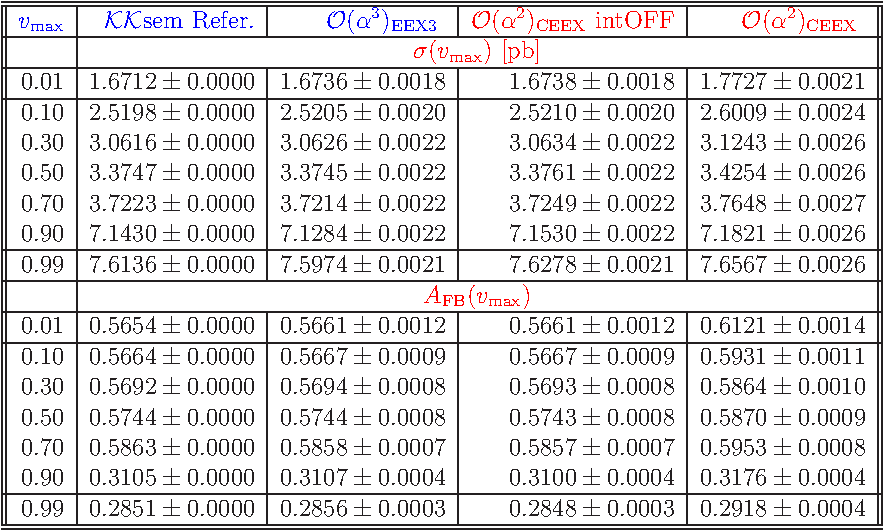
\includegraphics[width=90mm,height=60mm]{afb_int2-tab1.pdf}}

\small
Energy cut-off study of
total cross section  $\sigma$ and charge asymmetry $A_{\rm FB}$
for annihilation process $e^-e^+ \to \mu^-\mu^+$, at $\sqrt{s}=$189GeV.\\
Energy cut: $v<v_{\max}$, $v=1-M^2_{f\bar{f}}/s$.\\
From http://arxiv.org/abs/arXiv:1307.4037
\end{frame}
%----------------------------------------------------------------------


%----------------------------------------------------------------------
\begin{frame}[fragile]
\frametitle{\bf More on KKMC version 4.22 (2013)}
\framesubtitle{\bf\large Physics extensions, 1st step: lepton beams}
\vspace{-2mm}
\large
Lepton {\cbl beams $\neq e^\pm$}, 
for instance $\mu^-\mu^+,q\bar{q}$, etc.

{\footnotesize
Mainly the problem of transfering properly mass of beam leptons.
}\\
A few corrections, et voil\'a!
~~\fbox{\cbl $\mu^- \mu^+ \to e^- e^+$} at 189GeV.

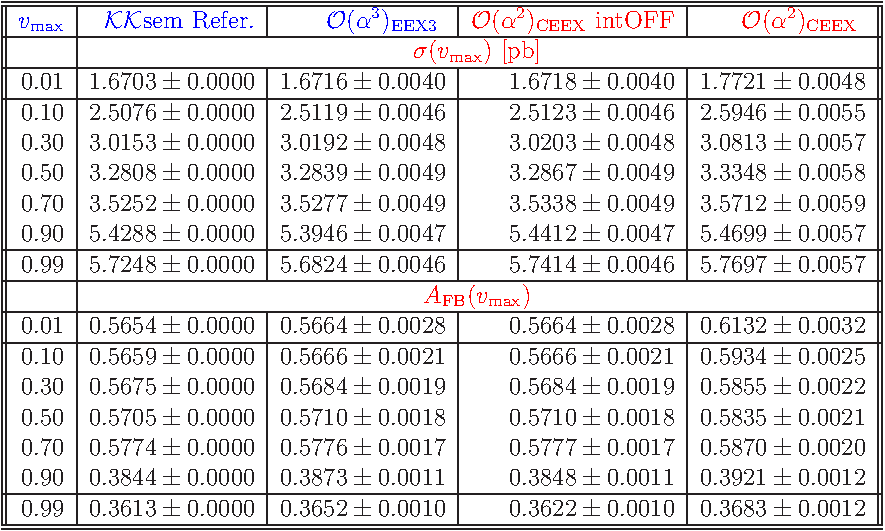
\includegraphics[width=90mm]{afb_int2-tab1-mu2e.pdf}

\end{frame}
%----------------------------------------------------------------------


%----------------------------------------------------------------------
\begin{frame}[fragile]
\frametitle{\bf More on KKMC version 4.22 (2013)}
\framesubtitle{\bf\large Physics extensions, 2nd step: quark beams}
\large
Quark {\cbl beams} at fixed energy.

{\footnotesize
Mainly the problem of transfering properly weak isospin of beams.
}\\
\fbox{\cbl $u \bar{u} \to e^- e^+ +n\gamma$}
at $\sqrt{s}=M_Z$. Again KKMC vs. KKsem.

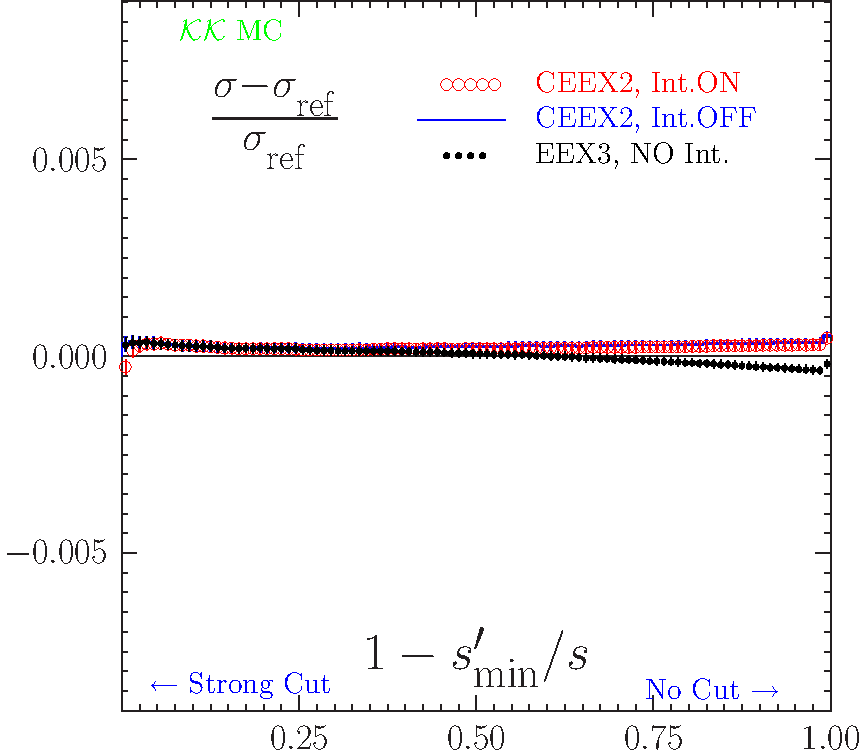
\includegraphics[width=70mm]{afb_int2-Gsig-u2mu-91.pdf}

\end{frame}
%----------------------------------------------------------------------


%----------------------------------------------------------------------
\begin{frame}[fragile]
\frametitle{\bf More on KKMC version 4.22 (2013)}
\framesubtitle{\bf\large Physics extensions, 3rd step: PDFs for quark beam}
\large
Quark {\cbl beams} at energies varying according to PDFs.

~~~\\
{\footnotesize
Main problem in the code: variable $\sqrt{s}$ from one MC event to another.\\
Luckily already solved for beamstrahlung.
}

~~~\\
Test for \fbox{\cbl $u \bar{u} \to e^- e^+ +n\gamma$}
at $\sqrt{s}=M_Z$.

~~~\\
KKMC vs. KKsem not available:(\\
Only kinematics was tested, see event printout next slide.

\end{frame}
%----------------------------------------------------------------------

%----------------------------------------------------------------------
\begin{frame}[fragile]
\frametitle{\bf More on KKMC version 4.22 (2013)}
\framesubtitle{\bf\large Physics extensions, 3rd step: PDFs for quark beam}

{\tiny
\baselineskip=3pt
\begin{verbatim}
 ***************************************************************************
 *                         KK Monte Carlo                                  *
 *            Version       4.22          May 2013                         *
 *    7000.00000000                 CMS energy average       CMSene     a1 *
 *       0.00000000                 Beam energy spread       DelEne     a2 *
 *              100                 Max. photon mult.        npmax      a3 *
 *                0                 wt-ed or wt=1 evts.      KeyWgt     a4 *
 *                1                 ISR switch               KeyISR     a4 *
 *                1                 FSR switch               KeyFSR     a5 *
 *                2                 ISR/FSR interferenc      KeyINT     a6 *
 *                1                 New exponentiation       KeyGPS     a7 *
 *                0                 Hadroniz.  switch        KeyHad     a7 *
 *       0.20000000                 Hadroniz. min. mass      HadMin     a9 *
 *       1.00000000                 Maximum weight           WTmax     a10 *
 *              100                 Max. photon mult.        npmax     a11 *
 *                2                 Beam ident               KFini     a12 *
 *       0.03500000                 Manimum phot. ener.      Ene       a13 *
 *   0.10000000E-59                 Phot.mass, IR regul      MasPho    a14 *
 *    1.2500000                     Phot. mult. enhanc.      Xenph     a15 *
 *       0.00000000                    PolBeam1(1)           Pol1x     a17 *
 *       0.00000000                    PolBeam1(2)           Pol1y     a18 *
 *       0.00000000                    PolBeam1(3)           Pol1z     a19 *
 *       0.00000000                    PolBeam2(1)           Pol2x     a20 *
 *       0.00000000                    PolBeam2(2)           Pol2y     a21 *
 *       0.00000000                    PolBeam2(3)           Pol2z     a22 *
 ***************************************************************************
  
                            Event listing (summary)
    I particle/jet KS     KF  orig    p_x      p_y      p_z       E        m
    1 !u!          21       2    0    0.000    0.000   22.668   22.668    0.005
    2 !ubar!       21      -2    0    0.000    0.000 -245.458  245.458    0.005
    3 (Z0)         11      23    1   23.016   18.370  -80.068  115.249   77.487
    4 gamma         1      22    1  -30.989   -6.132 -128.905  132.719    0.000
    5 gamma         1      22    1    0.000    0.000    0.031    0.031    0.000
    6 gamma         1      22    1    7.973  -12.238  -13.848   20.127    0.000
    7 gamma         1      22    1    0.000    0.000 3477.332 3477.332    0.000
    8 gamma         1      22    1    0.000    0.000-3254.542 3254.542    0.000
    9 tau-          1      15    3  -24.701   21.657  -20.217   38.613    1.777
   10 tau+          1     -15    3   47.716   -3.287  -59.851   76.635    1.777
                   sum:  0.00         0.000    0.000    0.000 7000.000 7000.000
\end{verbatim}
}% small
\end{frame}
%----------------------------------------------------------------------

%----------------------------------------------------------------------
\begin{frame}[fragile]
\frametitle{ Cont.}

{\tiny
\baselineskip=3pt
\begin{verbatim}
                            Event listing (summary)
    I particle/jet KS     KF  orig    p_x      p_y      p_z       E        m
    1 !u!          21       2    0    0.000    0.000  271.908  271.908    0.005
    2 !ubar!       21      -2    0    0.000    0.000   -6.542    6.542    0.005
    3 (Z0)         11      23    1    0.047    1.133  244.401  257.454   80.928
    4 gamma         1      22    1   -0.047   -1.133   20.965   20.996    0.000
    5 gamma         1      22    1    0.000    0.000 3228.092 3228.092    0.000
    6 gamma         1      22    1    0.000    0.000-3493.458 3493.458    0.000
    7 mu-           1      13    3    0.601   14.537    2.005   14.687    0.106
    8 mu+           1     -13    3   -0.554  -13.404  242.396  242.767    0.106
                   sum:  0.00         0.000    0.000    0.000 7000.000 7000.000

                            Event listing (summary)

    I particle/jet KS     KF  orig    p_x      p_y      p_z       E        m
    1 !u!          21       2    0    0.000    0.000 1816.851 1816.851    0.005
    2 !ubar!       21      -2    0    0.000    0.000   -1.137    1.137    0.005
    3 (Z0)         11      23    1    0.011    0.003 1810.259 1812.532   90.760
    4 gamma         1      22    1   -0.012   -0.002    5.371    5.371    0.000
    5 gamma         1      22    1    0.000    0.000 1683.149 1683.149    0.000
    6 gamma         1      22    1    0.000    0.000-3498.863 3498.863    0.000
    7 mu-           1      13    3   12.468  -25.466 1612.743 1612.992    0.106
    8 mu+           1     -13    3  -12.457   25.469  197.516  199.540    0.106
                   sum:  0.00        -0.001    0.001   -0.084 6999.916 6999.916


 ***************************************************************************
 *                       KK2f_Finalize  printouts                          *
 *    7000.00000000                 cms energy total         cmsene     a0 *
 *             5000                 total no of events       nevgen     a1 *
 *               ** principal info on x-section **                         *
 *     233.95163953  +- 1.04896414  xs_tot MC R-units        xsmc       a1 *
 *       0.41468908                 xs_tot    picob.         xSecPb     a3 *
 *       0.00185933                 error     picob.         xErrPb     a4 *
 *       0.00448368                 relative error           erel       a5 *
 *       0.82048782                 WTsup, largest WT        WTsup     a10 *
 *                       ** some auxiliary info **                         *
 *       0.00219522                 xs_born   picobarns       xborn    a11 *
 *       0.73760000                 Raw phot. multipl.                 === *
 *       5.00000000                 Highest phot. mult.                === *
 *                         End of KK2f  Finalize                           *
 ***************************************************************************

\end{verbatim}
}% small
\end{frame}
%----------------------------------------------------------------------


%----------------------------------------------------------------------
\begin{frame}[fragile]
\frametitle{\bf Possible other extensions?}
%\framesubtitle{Mission statement}

\small
Could one include/improve
QCD correction for the incoming beams?\\
Yes, for example classic NLO corrs, Powheg style etc.

~~~\\
In this case the upper level of KKMC would be replaced by C++ code,
which is already in place in some simple form.

~~~\\
The extension to $q\bar{q} \to W \to l+\nu$ is thinkable,
but would require update of the QED matrix element (EW corrs. ?)

~~~\\
NB. t-canel $W$ exchange with h.o. QED
is already there for $\nu\bar\nu$ chanel and could be exploited
as a starting point.

~~~\\
However, the bottom line still vailid is:\\
Let us exploit the existing KKMC as much as we can for LHC!!!
\end{frame}
%----------------------------------------------------------------------



%----------------------------------------------------------------------
\begin{frame}[fragile]
\frametitle{\bf\LARGE Summary}
%\framesubtitle{Mission statement}

\Huge
KKMC still alive and possibly still useful!

\end{frame}
%----------------------------------------------------------------------


\end{document}
%%%%%%%%%%%%%%%%%%%%%%%%%%%%%%%%%%%%%%%%%%%%%%%%%%%%%%%%%%%%%%%%%%%%%%%%
%%%%%%%%%%%%%%%%%%%%%%%%%%%%%%%%%%%%%%%%%%%%%%%%%%%%%%%%%%%%%%%%%%%%%%%%
%%%%%%%%%%%%%%%%%%%%%%%%%%%%%%%%%%%%%%%%%%%%%%%%%%%%%%%%%%%%%%%%%%%%%%%%
%%%%%%%%%%%%%%%%%%%%%%%%%%%%%%%%%%%%%%%%%%%%%%%%%%%%%%%%%%%%%%%%%%%%%%%%


%----------------------------------------------------------------------
\begin{frame}[fragile]
\frametitle{Abstract (plan of the talk)}
%\framesubtitle{Mission statement}
...
\end{frame}
%----------------------------------------------------------------------


